\scanpage{81}

$f$ convex function on the convex open set $U$,

\[
(x,y)\in G_f\iff x\in U\text{ and } y>f(x)
\]

Let \deleted{\unsure{$x_0,y_0$|$x,y$|$x_i,y_i$}} $(a,b)$ with $b=f(a)$ $(a\in U)$, \deleted{\unsure{thus|one}} let $H$ be a hyperplane passing through $(a,b)$ not meeting the open set $G_f$, then : 1) it is of the form

\[
y-b=\deleted{\unsure{\sum c_i x_i+\beta}}=\sum c_i(x_i-a_i)
\]

(for does not contain the line $x=a$), say $y=L_a(x)$

2) We have $f(x)\geq L(x)$ for \uline{\unsure{every|every}} $x\in U$ (indeed, one of the two \deleted{\unsure{hyperplanes}} \inserted{open} semi-spaces determined by $H$ contains $G_f$, and it can only be the one given by $y\geq L(x)$. \deleted{\unsure{thus}} whence the conclusion), 3) We have for $x\in E$ $f(x)=\sup_a L_a(x)$ (the sup being attained), and conversely. 4) If at the point $a$, $f(x)$ is increasing then the $c_i$ are $\geq0$. Indeed, if we had for example $c_1<0$, then $f(x_1,a_2,-a_n)$ is increasing at the point $x_1=a_1$,
\reversemarginpar\margin{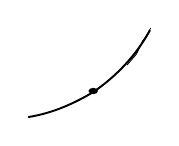
\begin{tikzpicture}[x=.1mm,y=-.1mm,line cap=round,line join=round]
\draw[line width=.7pt] (11,122) .. controls (42,117) and (68,105) .. (92,91) .. controls (122,71) and (148,43) .. (165,12);
\draw[line width=.25pt] (81,97) .. controls (105,84) and (129,63) .. (148,40) -- (166,9);
\draw[line width=.3pt] (136,56) -- (148,42) -- (156,25) -- (162,18);
\fill (93,89) ellipse (6 and 4);
\end{tikzpicture}}\normalmarginpar
and \deleted{of} bounded below by $L(x_1,a_2-a_n)$, linear function taking at the \unsure{point|point} $a$ the same value as $f$. The latter cannot be strictly decreasing for we would have $f(x_1)\leq f(a)\leq f(x_1)$ for $x_1<a_1$ near $a_1$.

\reversemarginpar\margin{82}\normalmarginpar
